% works on TeX-Live 2015

\documentclass{beamer}
\usepackage{tgheros}
\usepackage[varqu, scaled]{inconsolata}
\usepackage{mylistings}
\usepackage{csquotes}
\usepackage{hyperref}
\usepackage{tikz}
%\usepackage{tikz-uml}

\lstset{
  style=colored,
  %belowskip=0pt
  basicstyle=\ttfamily\small\color{darkgray},
  columns=[c]fixed,
  gobble=4
}

\usetheme[compress]{Singapore}
\setbeamercolor{structure}{fg=textblue}

% smaller footnotes; see: http://tex.stackexchange.com/a/192652/46356
\setbeamertemplate{footnote}{%
  \tiny%
  \parindent 1em\noindent%
  \raggedright
  \hbox to 1.8em{\hfil\insertfootnotemark}\insertfootnotetext\par%
}%
\setlength\footnotesep{0pt}

\author{Functional Programming Graz}
\title{Why Functional Programming Matters\footnote{Title stolen from
    \href{http://www.cse.chalmers.se/\~rjmh/Papers/whyfp.pdf}{(Hughes, 1984)}}}
\date{April 2016}

%%%%%%%%%%%%%%%%%%%%%%%%%%%%%%%%%%%%%%%%%%%%%%%%%%%%%%%%%%%%%%%%%%%%%%%%%%%%%%%%%%%%%%%%%%%%%%%%%%%%
\begin{document}

\begin{frame}
  \maketitle
\end{frame}

\section{Introduction}

\begin{frame}[containsverbatim]
  \frametitle{Functional programming is scary?}
  \begin{center}
    \href{https://upload.wikimedia.org/wikipedia/commons/9/9d/The_Scream_by_Edvard_Munch%2C_1893_-_Nasjonalgalleriet.png}{%
      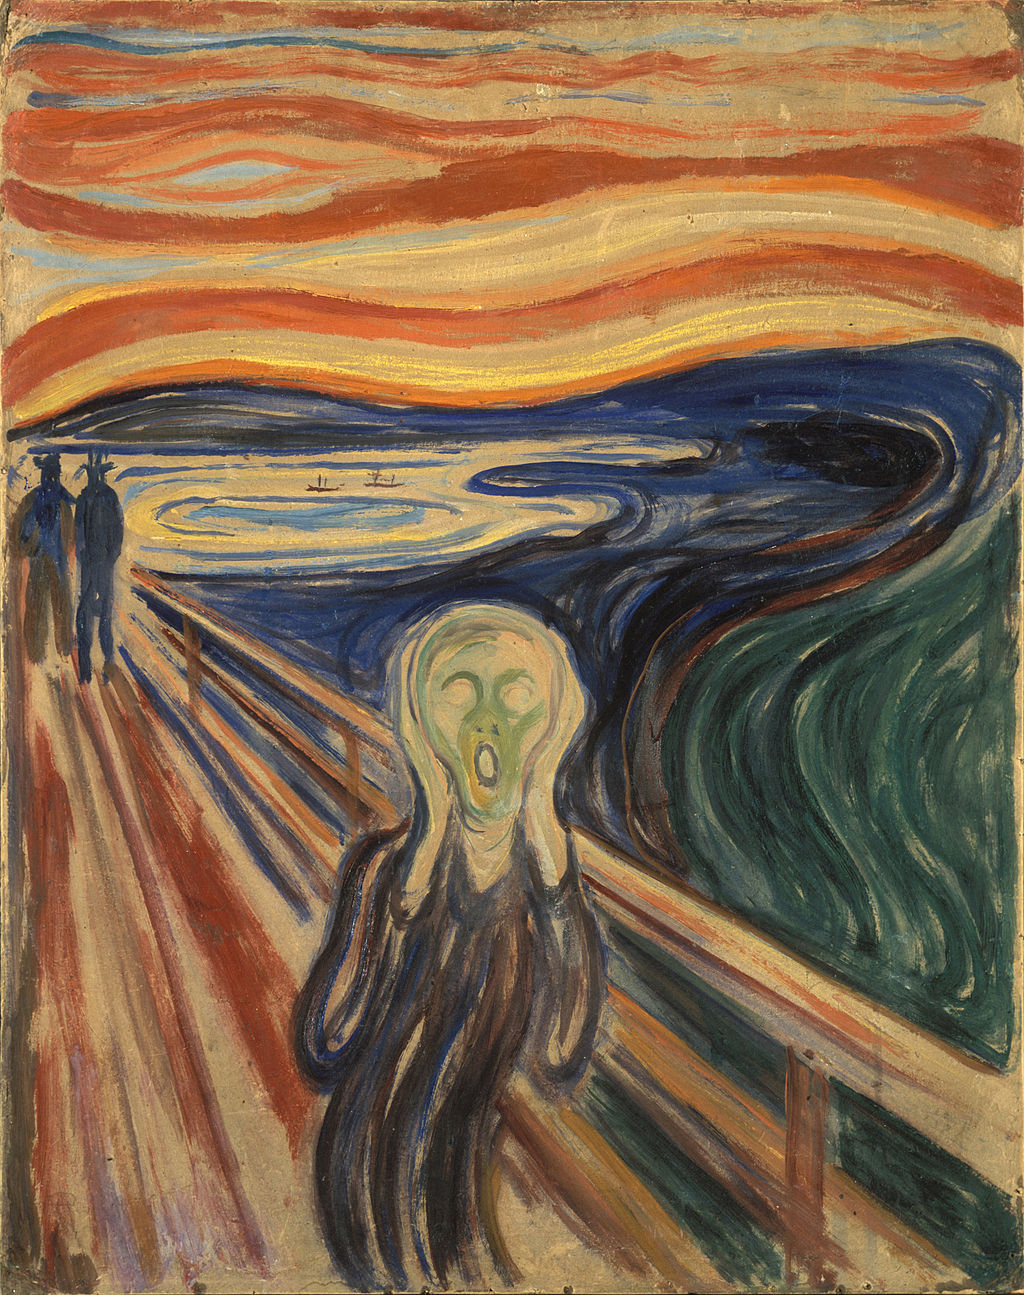
\includegraphics[height=0.7\textheight]{fig/munch}}
  \end{center}
\end{frame}

\begin{frame}[containsverbatim]
  \frametitle{Functional programming is scary?}
  Don't fear: we \textit{don't} mean code like this:\footnote{(Code by
    \href{http://www.willamette.edu/~fruehr/haskell/evolution.html}{Fritz Ruehr})}

  \begin{tikzpicture}
    \usetikzlibrary{shapes.misc}
    \node [] {\begin{lstlisting}{language=[Modern]Haskell, gobble=4}
    gcata :: (Functor f, Comonad n) =>
      (forall a. f (n a) -> n (f a)) 
        -> (f (n c) -> c) -> Mu f -> c
    gcata dist phi = extr . cata (fmap phi . dist . fmap dupl)

    zygo chi = gcata (fork (fmap outl) (chi . fmap outr))

    para :: Functor f => (f (Prod (Mu f) c) -> c) -> Mu f -> c
    para = zygo In
    \end{lstlisting}};
  \node (1,1) [cross out, draw=red, 
              line width=3pt, line cap=round,
              minimum width=10cm, minimum height=3cm] {};
  \end{tikzpicture}
\end{frame}

\begin{frame}[containsverbatim]
  \frametitle{No! (at least, mostly)} 

  Rather, we would like to focus on stuff that makes code \textit{more} readable:\footnote{%
    Note that in Haskell, function application works by juxtaposition, not parentheses; this is
    actually very useful with higher order functions.}

  \begin{lstlisting}{language=[Modern]Haskell}
    quicksort :: Ord a => [a] -> [a]
    quicksort [] = []
    quicksort (x:xs) = quicksort smaller 
                       ++ [x] 
                       ++ quicksort greater
      where smaller = [y | y <- xs, y <= x]
            greater = [y | y <- xs, y > x]
  \end{lstlisting}

  Of course, as with everything, you have to get used to it first. But\ldots
\end{frame}

\begin{frame}[containsverbatim]
  \frametitle{Functional programming can lead to enlightening!}

  \begin{center}
    \href{https://upload.wikimedia.org/wikipedia/commons/a/a7/Ferdinand_Bol_-_Moses_descends_from_Mount_Siniai_with_the_Ten_Commandments_-_Google_Art_Project.jpg}{%
      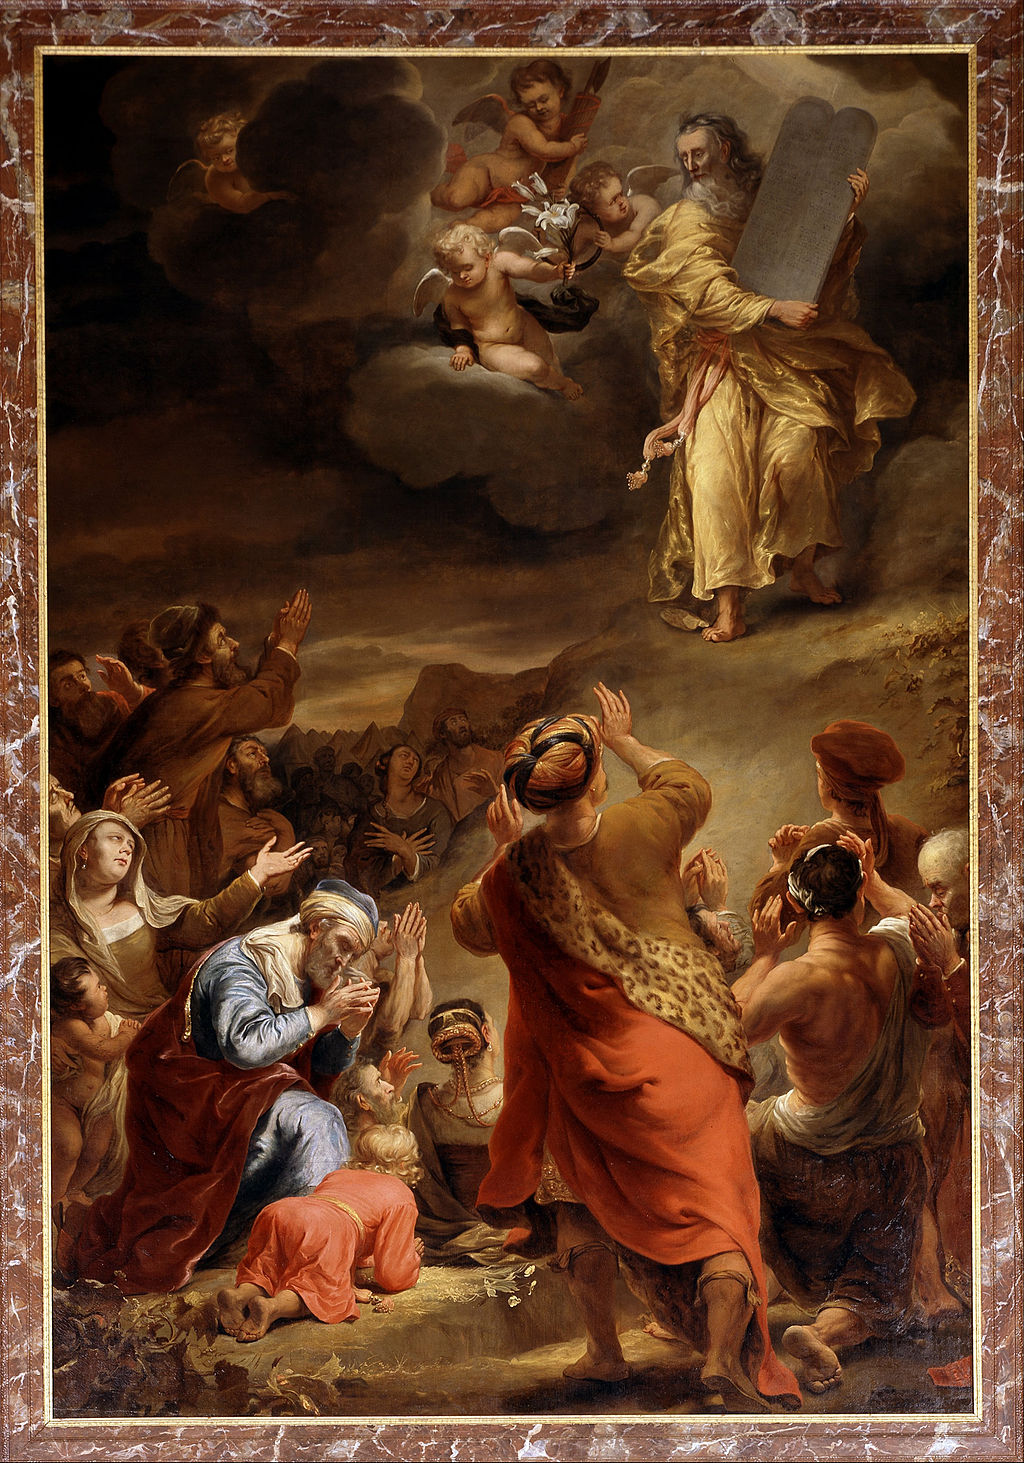
\includegraphics[height=0.7\textheight]{fig/bol}}
  \end{center}

  \ldots or at least, it will change you way of thinking and approaching problems in a positive way.
\end{frame}


\section{Higher-order functions}

\begin{frame}[containsverbatim]
  \frametitle{Higher-order functions to the rescue!} 

  If used in the right places, we can write more declarative and reusable code by using functions as
  values.

  \begin{lstlisting}{language=Python}
    union = reduce(or_, all_sets, set())
    hitting_sets = {p for p in powerset(union) 
                    if all(p & s for s in all_sets)}
  \end{lstlisting}

  Doing such things needs getting used to, and requires one to use much more recursion and less
  mutability than one normally would as an imperative programmer, but the resulting style has a lot
  of advantages.
\end{frame}


\begin{frame}[containsverbatim]
  \frametitle{Remember pipe \& filter?} 

  The usual example of stream processing: passing functions into \lstinline|map|,
  \lstinline|filter|, friends:\footnote{(Code by
    \href{http://www.oracle.com/technetwork/articles/java/ma14-java-se-8-streams-2177646.html}{%
      Raoul-Gabriel Urma)}}

  \begin{lstlisting}{language=Java}
    transactions.stream()
                .filter(t -> 
                  t.getType() == Transaction.GROCERY)
                .sorted(comparing(Transaction::getValue)
                        .reversed())
                .map(Transaction::getId)
                .collect(toList());
  \end{lstlisting}

  Although this quickly gets boring\ldots but we can also do \enquote{non-linear} things.
\end{frame}

\begin{frame}[containsverbatim]
  \frametitle{Streams for more complex list processing} 

  This expression does overload resolution for function arguments:

  \begin{lstlisting}{language=Java}
    overloads.stream()
      .flatMap(o -> applicationCostFor(arguments, o.input)
                    .map(c -> Stream.of(Pair.of(o.output, c)))
                    .orElse(Stream.empty()))
      .sorted(Comparator.comparing(p -> p._2))
      .map(p -> p._1)
      .findFirst();
  \end{lstlisting}

  \lstinline|flatMap| allows to filter and map at the same time; also, using \lstinline|map| on 
  \lstinline|Optional|s (\lstinline|applicationCostFor| returns an \lstinline|Optional<Int>|) makes
  this one safe, self-contained expression.
\end{frame}



\begin{frame}[containsverbatim]
  \frametitle{Lazy streams} 
  
  This gets much more interesting if we use non-strict evaluation:

  \begin{lstlisting}{language=[Modern]Haskell}
    Prelude> let fibs = 0 : 1 : zipWith (+) fibs (tail fibs)
    Prelude> take 10 fibs
    [0,1,1,2,3,5,8,13,21,34]
  \end{lstlisting}

  Yes, that is a recursively defined list of infinite length.\footnote{Although this is inefficient;
    but there is an almost equivalent memoized\\ version requiring only linear time and space.}
\end{frame}

\begin{frame}[containsverbatim]
  \frametitle{\textit{Reactive} streams} 

  Taking this to the extreme, we arrive at reactive programming:\footnote{(Code by
    \href{https://gist.github.com/staltz/868e7e9bc2a7b8c1f754}{%
      Andre Medeiros)}}

  \begin{lstlisting}
    var refreshClickStream = 
      Rx.Observable.fromEvent(refreshButton, 'click');
    var requestStream = refreshClickStream
      .startWith('startup click')
      .map(function() {
        var randomOffset = Math.floor(Math.random() * 500);
        return 'https://api.github.com/users?since=' 
          + randomOffset;
      });
      .flatMap(function (requestUrl) {
        return Rx.Observable.fromPromise(
          $.ajax({url: requestUrl}));
      });
  \end{lstlisting} % $

  
\end{frame}

\begin{frame}[containsverbatim]
  \frametitle{Function chaining in R (\texttt{dplyr})} 

  There is also a certain relationship with query languages; however, we can mix in arbitrary custom
  functions. This is a way to describe operations on data frames (in-memory, or possibly in a
  database):\footnote{(Code from the \texttt{dplyr} 
    \href{https://cran.r-project.org/web/packages/dplyr/vignettes/introduction.html}{vignette})}

  \begin{lstlisting}{language=R}
    flights %>%
      group_by(year, month, day) %>%
      select(arr_delay, dep_delay) %>%
      summarise(arr = mean(arr_delay), 
                dep = mean(dep_delay)) %>%
      filter(arr > 30 | dep > 30) %>% 
      ggplot(aes(factor(month), arr + dep)) + geom_boxplot()
  \end{lstlisting}

  \lstinline|x %>% f(y)| is turned into \lstinline|f(x, y)|. We see that this pattern relies on
               immutability and partial application.
\end{frame}

\begin{frame}[containsverbatim]
  \frametitle{Function chaining in R (\texttt{dplyr})} 
  Result:
  \begin{center}
    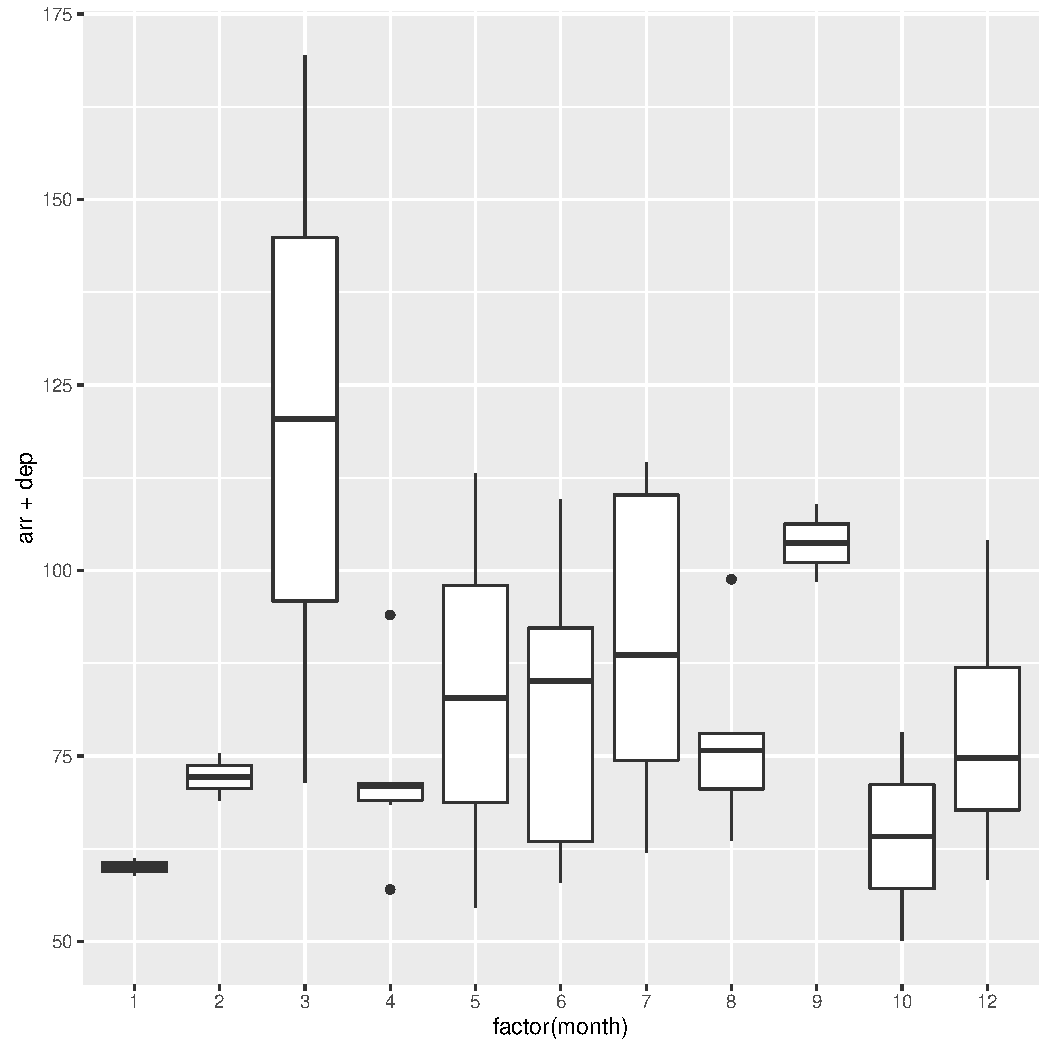
\includegraphics[height=0.7\textheight]{fig/plot}
  \end{center}
\end{frame}



\begin{frame}[containsverbatim]
  \frametitle{Property-based testing} 

  Testing by specification of invariants:

  \begin{lstlisting}{language=Scala}
    val propReverseList = forAll {
      l: List[String] => l.reverse.reverse == l
    }

    val propConcatString = forAll {
      (s1: String, s2: String) => (s1 + s2).endsWith(s2)
    }
  \end{lstlisting}

  This is \textit{not} a unit test~-- instead, the predicate is applied to a lot of randomly
  generated values of its input types.

  How is \lstinline|forAll| implemented? Purely as a library
  function!\footnote{See: \protect\url{http://www.scalacheck.org/}}
\end{frame}


\section{Data transformations}

\begin{frame}[containsverbatim]
  \frametitle{Algebraic data types (ADTs)} 

  \ldots are lightweight and extremely useful. Especially, we have \textit{sum types} (aka
  \enquote{tagged unions}). They are used through pattern matching:

  \begin{lstlisting}{language=[Modern]Haskell}
    data Bool = True | False

    (||) :: Bool -> Bool -> Bool
    True || something = True
    False || something = False

    data Tree a = Leave a | Branch (Tree a) (Tree a)

    contains :: (a -> Bool) -> Tree a -> Bool
    contains p (Leave a) = p a
    contains p (Branch l r) = contains p l || contains p r 
  \end{lstlisting}

  (As visible in the type, \lstinline|p| is a predicate, ie. a function from \lstinline|a| to
  \lstinline|Bool|.)
\end{frame}

\begin{frame}[containsverbatim]
  \frametitle{Option: the better \texttt{null}} 

  Now, what if we also want to get the matched value, not only find out whether it's there? We must
  be careful, since maybe there is no value at all. To represent that option, we use
  \lstinline|Option|:

  \begin{lstlisting}{language=[Modern]Haskell}
    data Option a = Nothing | Just a

    find :: (a -> Bool) -> Tree a -> Option a
    find p (Leave a) = if p a then Just a
                       else Nothing
    find p (Branch l r) = case (find p l) of
      Just x -> Just x
      Nothing -> find p r
  \end{lstlisting}
\end{frame}

\begin{frame}[containsverbatim]
  \frametitle{Option: the better \texttt{null}} 

  But this nesting quickly gets tedious. Therefore: combinators, and more syntax.

  \begin{lstlisting}{language=[Modern]Haskell}
    find' :: (a -> Bool) -> Tree a -> Option a
    find' p (Leave a) | (p a) = Just a
                      | otherwise = Nothing
    find' p (Branch l r) = (find p l) <|> (find p r)
  \end{lstlisting}

  The (custom) operator \lstinline$<|>$ takes the left value, if it is not \lstinline|Nothing|, and
  otherwise returns the right side:

    \begin{lstlisting}{language=[Modern]Haskell}
    (<|>) :: Optional a -> Optional a -> Optional a
    (Just x) <|> something = Just x
    Nothing <|> something = something
  \end{lstlisting}
\end{frame}

\begin{frame}[containsverbatim]
  \frametitle{ADTs in object orientation} 

  Scala nicely integrates algebraic data types into its object oriented type system:

  \begin{lstlisting}{language=Scala}
    sealed trait Expr
    case class Var(name: String) extends Expr
    case class App(l: Expr, r: Expr) extends Expr
    case class Lambda(param: String, body: Expr) extends Expr

    def freeVarsOf(e: Expr): Set[String] = e match {
      case Var(x) => Set(x)
      case App(t1, t2) => freeVarsOf(t1) ++ freeVarsOf(t2)
      case Lambda(x, t) => freeVarsOf(t) - x
    }
  \end{lstlisting}
\end{frame}


\section{Type systems}

\begin{frame}[containsverbatim]
  \frametitle{Let the compiler do the work for you} 

  It's not like non-functional languages wouldn't have powerful type systems, too:\footnote{%
    (Code by \href{http://eli.thegreenplace.net/2014/variadic-templates-in-c/}{Ellen Bendersky})}

  \begin{lstlisting}{language=C++}
    template<typename T>
    T adder(T v) {
      return v;
    }

    template<typename T, typename... Args>
    T adder(T first, Args... args) {
      return first + adder(args...);
    }
  \end{lstlisting}

  But note that the above code is extremely funtional. In fact, the research about type systems is
  closely related to functional programming, since these two concepts naturally play well
  together~-- whereas in many imperative languages, sophisticated types are more like a construct
  put upon them after the fact.
\end{frame}

% \begin{frame}[containsverbatim]
%   \frametitle{} 

%   \begin{lstlisting}{language=C++}
%      /** Converts a function into a universally quantified property */
%      def forAll[A1,P](f: A1 => P)(implicit
%        p: P => Prop,
%        a1: Arbitrary[A1], 
%        s1: Shrink[A1], 
%        pp1: A1 => Pretty
%   ): Prop = forAllShrink(arbitrary[A1],shrink[A1])(f andThen p)
%   \end{lstlisting}

% \end{frame}













\begin{frame}[containsverbatim]
  \frametitle{} 

  \begin{lstlisting}{language=C++}
    
  \end{lstlisting}

\end{frame}

\end{document}